%%%%%%%%%%%%%%%%%%%%%%%%%%%%%%%%%%%%%%%%%
% Focus Beamer Presentation
% LaTeX Template
% Version 1.0 (8/8/18)
%
% This template has been downloaded from:
% http://www.LaTeXTemplates.com
%
% Original author:
% Pasquale Africa (https://github.com/elauksap/focus-beamertheme) with modifications by 
% Vel (vel@LaTeXTemplates.com)
%
% Template license:
% GNU GPL v3.0 License
%
% Important note:
% The bibliography/references need to be compiled with bibtex.
%
%%%%%%%%%%%%%%%%%%%%%%%%%%%%%%%%%%%%%%%%%

%----------------------------------------------------------------------------------------
%	PACKAGES AND OTHER DOCUMENT CONFIGURATIONS
%----------------------------------------------------------------------------------------

\documentclass{beamer}

\usetheme[numbering=none]{focus} % Use the Focus theme supplied with the template
% Add option [numbering=none] to disable the footer progress bar
% Add option [numbering=fullbar] to show the footer progress bar as always full with a slide count

% Uncomment to enable the ice-blue theme
%\definecolor{main}{RGB}{92, 138, 168}
%\definecolor{background}{RGB}{240, 247, 255}

%------------------------------------------------

\usepackage{booktabs} % Required for better table rules

%----------------------------------------------------------------------------------------
%	 TITLE SLIDE
%----------------------------------------------------------------------------------------


\title{PHPokémon}

\author{Frank van den Berg \\ Robin van der Noord \\ Victor Zwart \\ Wessel Poelman}

\titlegraphic{
\includegraphics[scale=0.3]{Images/PHPokemon.png}} % Optional title page image, comment this line to remove it

\date{19-06-2019}

%------------------------------------------------

\begin{document}

%------------------------------------------------

\begin{frame}
	\maketitle % Automatically created using the information in the commands above
\end{frame}

%----------------------------------------------------------------------------------------
%	 SECTION 1
%----------------------------------------------------------------------------------------
\section{De game} % Section title slide, unnumbered

\begin{frame}{Doelen:}
	\begin{itemize}
		\item 1 tegen 1 
		\item Keuze verschillende Pokémon
		\item Attack of switch
		\item Authentieke informatie gebruiken {\tiny(speed, defense, power, element, type, accuracy)}
		\item Simpele, begrijpelijke interface
	\end{itemize}
\end{frame}

%------------------------------------------------

\begin{frame}{Voorproefje}
	\begin{columns}
		\column{0.5\textwidth}
			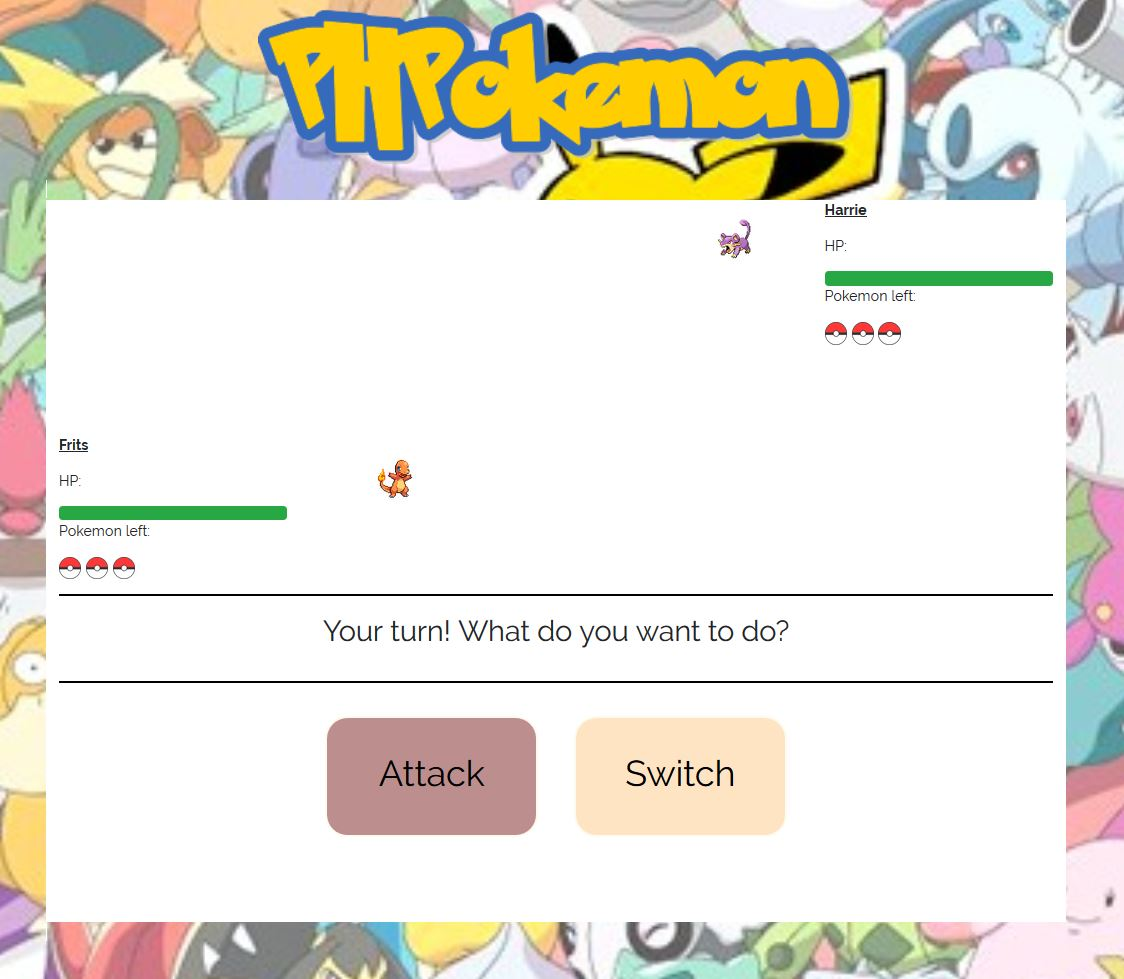
\includegraphics[width=\linewidth]{Images/screenshot2.jpg}
		
		\column{0.5\textwidth}
			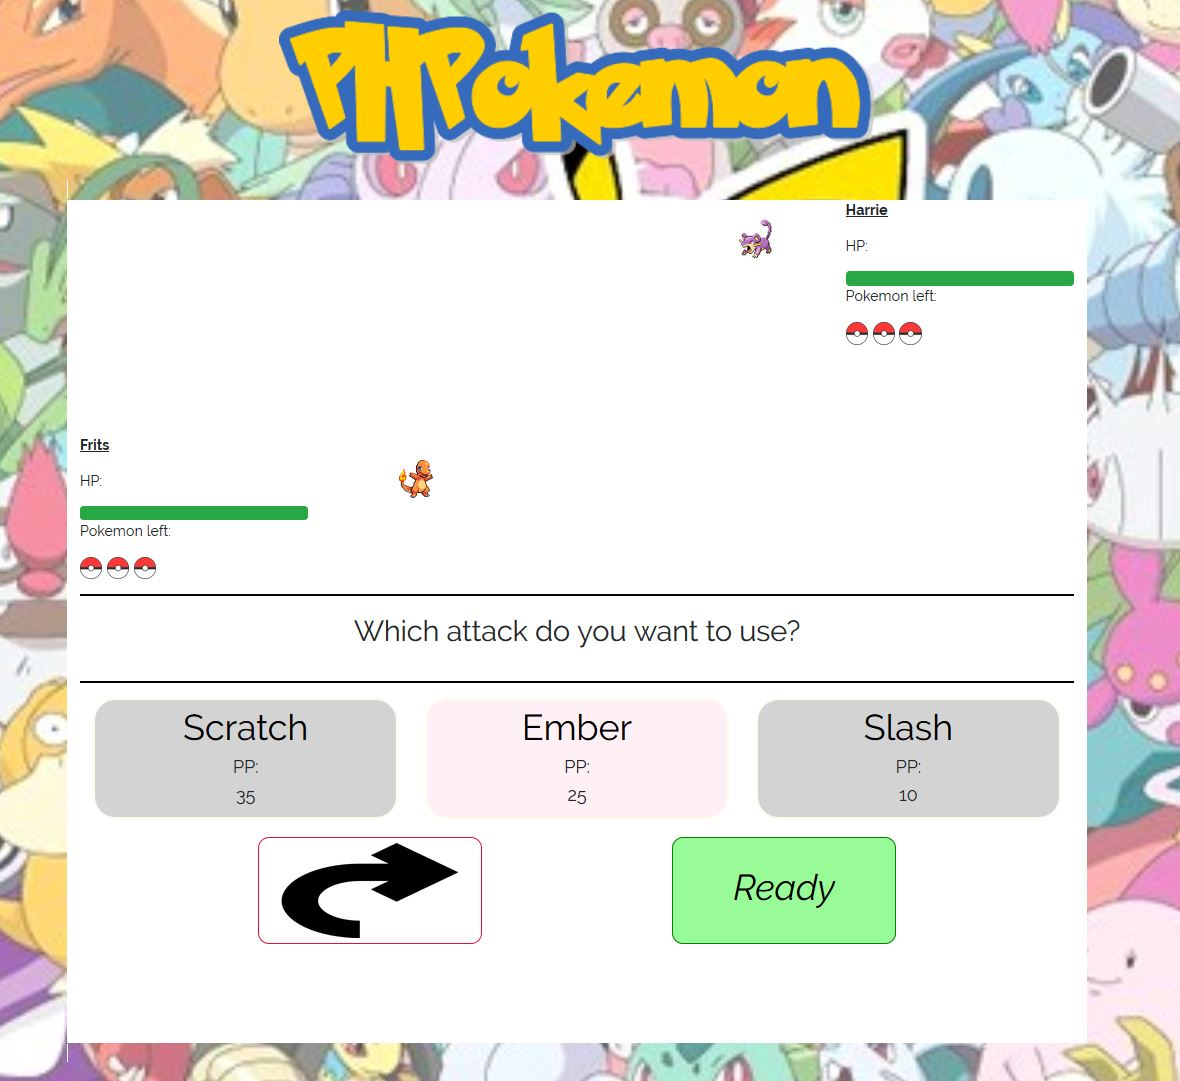
\includegraphics[width=\linewidth]{Images/screenshot3.jpg}

	\end{columns}
\end{frame}

%----------------------------------------------------------------------------------------
%	 SECTION 2
%----------------------------------------------------------------------------------------

\section{Methode}


\begin{frame}{Structuur}
	\begin{columns}
		\column{0.5\textwidth}
			\begin{itemize}
				\item MVC opbouw
				\item Routes
				\item Templating 
			\end{itemize}
		\column{0.5\textwidth}
			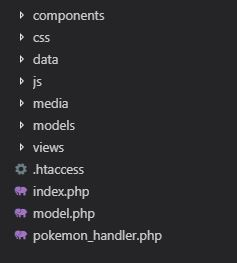
\includegraphics[scale=0.5]{Images/file_structure.jpg}
	\end{columns}
\end{frame}

%------------------------------------------------

\begin{frame}{Routes \& Controllers}
	
	\begin{itemize}
		\item \texttt{index.php} : statische GET routes
		\item \texttt{pokemon\textunderscore handler.php} : game GET \& POST routes
	\end{itemize}
\end{frame}

%------------------------------------------------

\begin{frame}{Models}
	\centering
	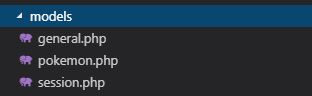
\includegraphics[scale=0.5]{Images/models.jpg}
	\begin{exampleblock}{general}
		Navigatie, routes, errors \& helpers.
	\end{exampleblock}
	\pause
	\begin{exampleblock}{pokemon}
		Round action ( (auto)switch, attack) \& damage.
	\end{exampleblock}
	\pause % Automatically creates a new "page" split between the above and above + below
	\begin{exampleblock}{session}
		Gamestate, reset game, player data \& join game.
	\end{exampleblock}
\end{frame}

%------------------------------------------------

\begin{frame}{Views}
	\begin{columns}
		\column{0.6\textwidth}
			\begin{itemize}
				\item Statische views (instructies \& Pokémon lijst)
				\item Components worden in 'main' geladen
				\item Component interactie \& dynamische data door Javascript
			\end{itemize}
		\column{0.4\textwidth}
			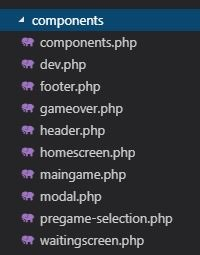
\includegraphics[scale=0.5]{Images/components.jpg}
			
\includegraphics[scale=0.5]{Images/views.jpg}
			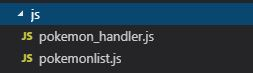
\includegraphics[scale=0.5]{Images/js.jpg}
	\end{columns}
\end{frame}
%------------------------------------------------

\begin{frame}{Interface}
	\begin{columns}
		\column{0.5\textwidth}
			\begin{itemize}
				\item Grote, duidelijke knoppen
				\item User feedback \\(animaties, omlijning, veranderen grootte)
				\item `Main game screen' met losse componenten
			\end{itemize}
		\column{0.5\textwidth}
			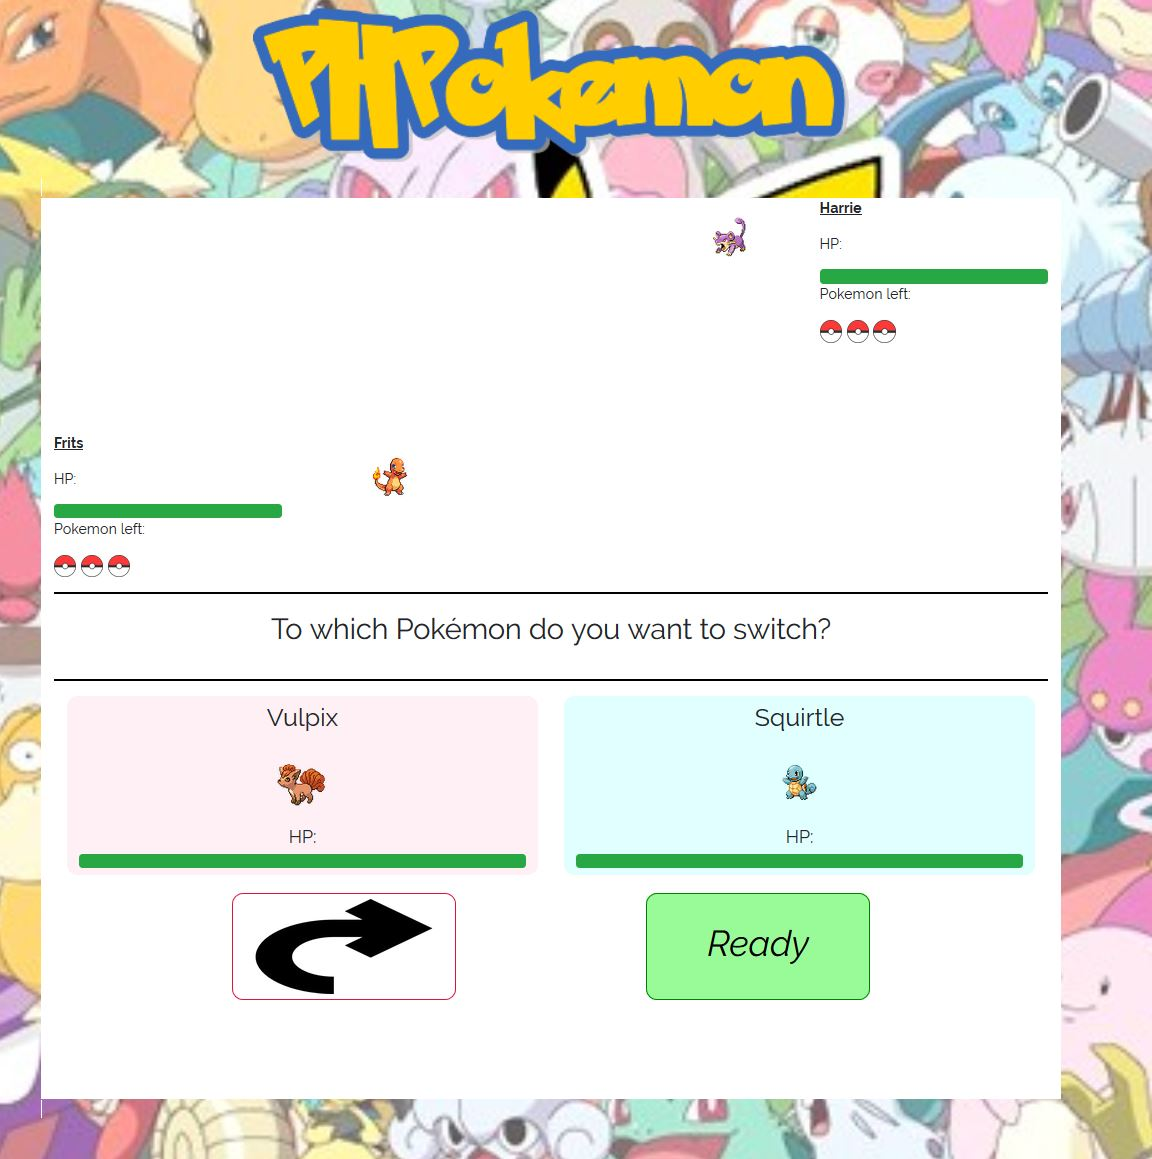
\includegraphics[scale=0.2]{Images/screenshot4.jpg}
	\end{columns}
\end{frame}

%------------------------------------------------

\begin{frame}{Data storage}
	\begin{columns}
		\column{0.7\textwidth}
			\hspace{50pt}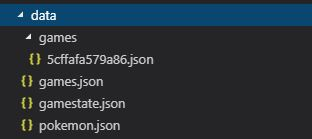
\includegraphics[scale=0.5]{Images/data.jpg} \\
			\bigskip
			\begin{itemize}
				\item \texttt{pokemon.json} : statische pokémon info
				\item \texttt{game\textunderscore state.json} : huidige game info (players, pokemon, data vorige rounds)
				\item \texttt{games.json} : id's van games die nu gespeeld worden (players, active?)
			\end{itemize}
		\column{0.3\textwidth}
			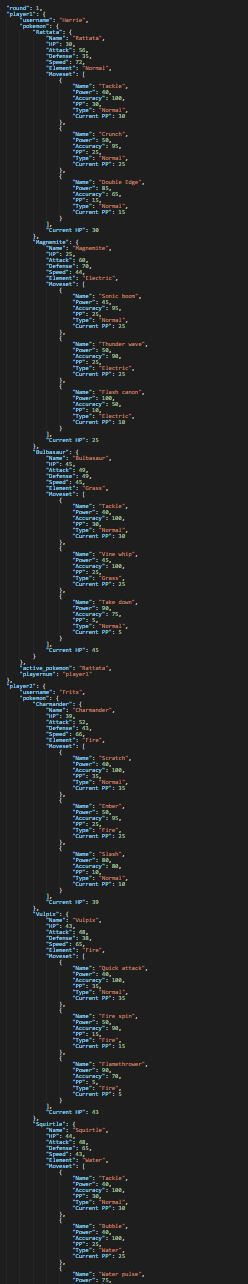
\includegraphics[scale=0.2]{Images/json.jpg}
	\end{columns}
\end{frame}

%------------------------------------------------

\begin{frame}{Taakverdeling}
	\begin{table}
		\centering % Centre the table on the slide
		\begin{tabular}{l l}
			Frank & {\tiny Interface, Animaties, Feedback messages, Pokémon lijst pagina, Damage berekenen}\\
			Robin & {\tiny Routing, Gamestate handling back-end, Errors, Players, Sessions}\\
			Victor & {\tiny Interface, Animaties, Sprites, Styling, Components}\\
			Wessel & {\tiny Gamestate handling front-end, Components, Errors}\\
			\midrule
			& \textbf{En elkaar helpen natuurlijk!} \\
			\bottomrule
		\end{tabular}
	\end{table}
\end{frame}

%------------------------------------------------

\begin{frame}{Git}
	\centering
	Een paar grote commits of veel kleine... Dat is de vraag...\\
	\bigskip
	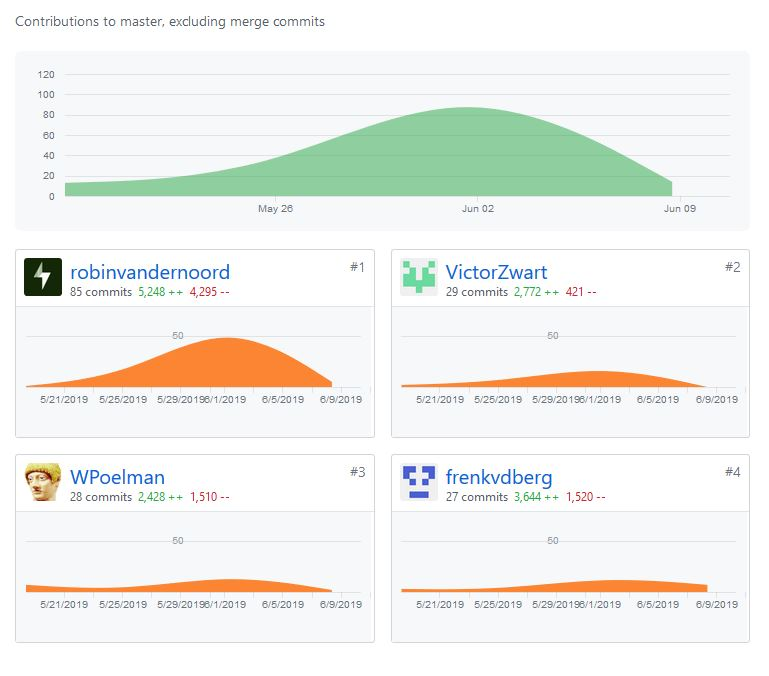
\includegraphics[scale=0.3]{Images/git.jpg}
\end{frame}

%------------------------------------------------

\begin{frame}[focus]
	\textbf{Demo}
\end{frame}

\end{document}
